\begin{frame}
  \frametitle{Conclusion}
  \begin{columns}
    \column[t]{5cm}
    \begin{enumerate}
      \item Replacing ``ABBOTT'' with nuclear would resolve all of the Universities
      carbon goals, \textit{regardless of other offsets and building growth.}
      \item Adding, even limited, nuclear capacity will cost effectively meet carbon goals until mid-decade.
      \item This model is agnostic to implementation:
      \begin{itemize}
        \item One 100 MWth small modular reactor
        \item Series of 20 MWth micro-reactors
      \end{itemize}
    \end{enumerate}
    \column[t]{5cm}
    \begin{figure}
      \centering
      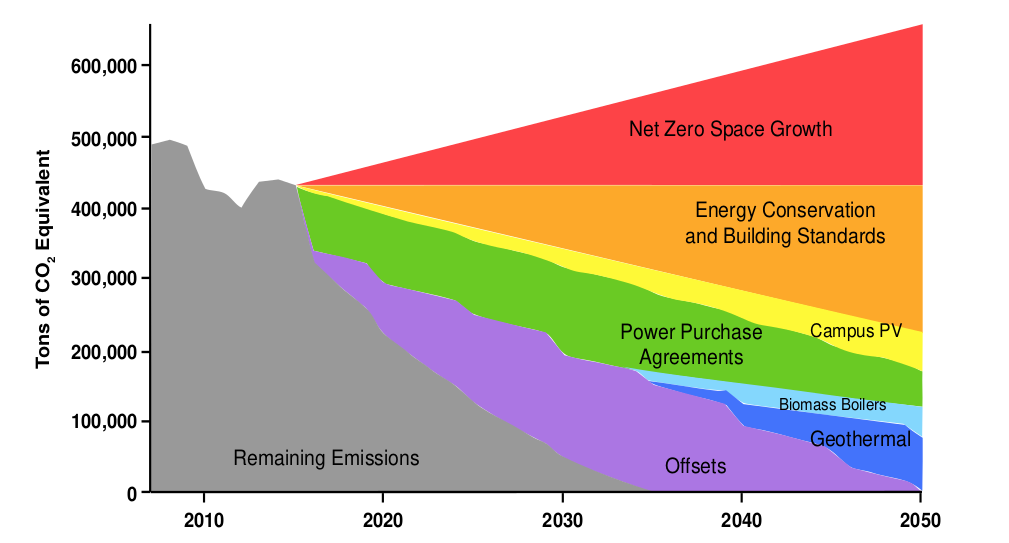
\includegraphics[width=\textwidth]{icap_uiucemissions.png}
      \caption{Shows projected CO$_2$ emissions for UIUC \cite{isee_illinois_2015}. Offsets include shutdown of the Blue Waters Supercomputer.}
      \label{fig:co2projections}
    \end{figure}
  \end{columns}
\end{frame}
